\chapter{Nanogeles polim\'ericos: Soluciones coloidales} \label{chapter:mc:soluciones}
	

	
	\section{Introducci\'on}
	
	Las soluciones coloidales de nanogeles polim\'ericos han ganado creciente atenci\'on recientemente  debido a sus propiedades y aplicaciones en varios campos. Los nanogeles son part\'iculas polim\'ericas reticuladas con dimensiones en el rango coloidal \cite{10.1002/pola.27653}. Estas part\'iculas combinan las propiedades de los pol\'imeros y de los coloides, como su capacidad de dispersar la luz, adquiriendo propiedades \'opticas \'unicas, o su capacidad de absorber cierta cantidad de solvente en el que se encuentran, en particular en medios biol\'ogicos les permite ser utilizados en aplicaciones biom\'edicas \cite{lyon2012polymer}. Los nanogeles son part\'iculas blandas, deformables y permeables con una estructura formada por una red polim\'erica. \cite{lyon2012polymer}. En soluci\'on, pueden absorber el solvente y expandir su volumen significativamente hacia un estado de baja densidad de pol\'imero \cite{karg2019nanogels, perez2021thermodynamic}. La concentraci\'on de part\'iculas de estas soluciones posee influencia en su estabilidad,  modificando su solubilidad en agua y tama\~no \cite{10.3390/polym13234071}. 
	
	Las soluciones coloidales de nanogeles son capaces de responder a diversos est\'imulos externos como la temperatura, la presi\'on, el pH, la fuerza i\'onica y la presencia de biomol\'eculas.
	La intrincadeza de esta respuesta genera una mayor complejidad en cualquier dispersi\'on compuesta por las mismas \cite{lyon2012polymer}.
	En este sentido, adem\'as de conocer como responden los nanogeles a diversos est\'imulos, es necesario estudiar c\'omo se ve modificada la respuesta de estas part\'iculas cuando forman soluciones coloidales relativamente concentradas. 
	
	La  capacidad de responder a diferentes est\'imulos externos esta definida por la composici\'on de la red polim\'erica. Los nanogeles compuestos por cadenas de pol\'imero que contienen segmentos \'acidos como \'acido acr\'ilico o metacr\'ilico (AA y MAA, respectivamente) se expanden o comprimen en respuesta a cambios en el pH de la soluci\'on \cite{snowden1996colloidal, Zhou1998}. Por otro lado nanogeles compuestos pol\'imeros termosensibles, por ejemplo PNIPAm, experimentan una transici\'on de fase volum\'etrica cuando se calientan por encima de una temperatura caracter\'istica \cite{Pelton1986, Pelton2000}. Este comportamiento se origina porque estos pol\'imeros son insolubles en agua por encima de su temperatura cr\'itica m\'inima de solubilidad (LCST, por sus siglas en ingl\'es) \cite{Kawaguchi2020}.
	
	Este tipo de  transiciones, tanto en respuesta al pH como a la temperatura, son reversibles. Es decir, si se aplica el est\'imulo externo en una direcci\'on provocando la expansi\'on de la part\'icula (swelling), la aplicaci\'on del est\'imulo en direcci\'on opuesta resulta en la compresi\'on del nanogel (deswelling).
	La incorporaci\'on de co-mon\'omeros termosensibles y con respuesta al pH a la red polim\'erica permite la obtenci\'on de nanogeles multi-responsivos, los cuales son atractivos para el dise\~no de sistemas inteligentes que funcionen en diferentes \'areas de la tecnolog\'ia \cite{plamper2017functional}. Se han estudiado microgeles de copol\'imeros de NIPAm y \'acido metacr\'ilico (MAA) \cite{Dowding2000, Hoare2004, Giussi2015}, encontr\'andose que su temperatura de cambio de fase depende del pH de la soluci\'on, la concentraci\'on de sal y la fracci\'on de mon\'omero ionizable en las cadenas de pol\'imero \cite{Morris1997, Jones2000, Hoare2004, Bradley2005, Lee2008, Wong2009, Hamzavi2016}. La incorporaci\'on del co-mon\'omero de MAA proporciona un mecanismo controlado por el pH para la adsorci\'on/liberaci\'on de mol\'eculas de carga de signo opuesto, lo que hace que los microgeles multiresponsivos sean atractivos para el dise\~no de diversos sistemas, entre ellos la administraci\'on de medicamentos \cite{Liu2017}.
	
	%En otros trabajos \cite{scotti2022softness, urich2016swelling} se han enfoncado en el estudio de la  arquitectura y composici\'on de los hidrogeles, lo que permite adaptar estas part\'iculas para que posean propiedades espec\'ificas.
	Las soluciones coloidales de nanogeles han sido estudiadas mediante simulaciones computacionales considerando  part\'iculas esf\'ericas que interact\'uan \'unicamente con un potencial de esferas duras \cite{karg2019nanogels}.
	 \citet{alziyadi2023osmotic} hizo uso de simulaciones de din\'amica molecular con una teor\'ia de Poisson-Boltzmann para estudiar microgeles cargados superficialmente. En otros estudios se ha hecho \'enfasis en soluciones con concentraciones altas de microgeles, en las cuales las part\'iculas se empaquetan densamente y forman una fase cristalina o amorfa  \cite{scotti2022softness, scheffold2020pathways}. La capacidad de comprimirse y formar diferentes fases de los nano/microgeles se convierte en un aspecto clave que influye en sus interacciones.
	Todas estas propiedades, incluida su estabilidad coloidal, convierte a los nanogles polim\'ericos en candidatos prometedores para una amplia gama de aplicaciones tales como biosensores \cite{zhang2012ultrathin, islam2014responsive}, ingenier\'ia de tejidos \cite{matricardi2013interpenetrating, van2011biopolymer}, regeneraci\'on \'osea \cite{bai2018bioactive}, materiales biomim\'eticos \cite{green2016mimicking, wu2010multifunctional}, entre muchas otras aplicaciones biom\'edicas \cite{Daly2020}.
	
	El cap\'itulo \ref{Chapter-geles} se dedic\'o al desarrollo de una teor\'ia termodin\'amica para el entendimiento de microgeles con respuesta a la temperatura, pH y concentraci\'on de sal. Los resultados presentados en dicho cap\'itulo describen la fisicoqu\'imica detr\'as de los fen\'omenos del swelling de estos microgeles impulsada por el pH y la dependencia no mon\'otona del tama\~no de part\'icula con la concentraci\'on de sal. 
	En este cap\'itulo damos un paso  adelante mostrando un estudio sistem\'atico de soluciones coloidales compuestos por nanogeles de P(NIPAm-co-MAA). Para este prop\'osito se har\'a uso de una metodolog\'ia basada en simulaciones Monte Carlo en el cual se combinan potenciales de interacci\'on part\'icula-part\'icula y de la termodin\'amica de intra-nanogel desarrollada en \cite{perez2021thermodynamic}. 
	
	%%%% aqui motivación del capitulo
	%%% lo que sigue es lo que se hace, no la motivación.
	
	En este nuevo cap\'itulo se incorporan potenciales entre part\'iculas de la soluci\'on de tal forma de estudiar la respuesta a est\'imulo de las soluciones de nanogeles como funci\'on de la concentraci\'on de sus part\'iculas. Estos potenciales buscan incorporar la naturaleza de los nanogeles de trabajo: su permeabilidad, capacidad de absorber solvente y adquirir carga el\'ectrica.

	%Por un lado, se agrega el potencial de Hertz, el cual tiene en cuenta la elasticidad de los nanogeles, lo que permite describir su capacidad de deformarse.
	%El potencial de Yukawa se puede utilizar para describir la interacci\'on electrost\'atica entre dos part\'iculas (nanogeles) cargadas teniendo en cuenta su carga el\'ectrica y las condiciones del medio en el que se encuentran, espec\'ificamente la fuerza i\'onica del medio.
	%El uso de estos potenciales permite describir los efectos que tiene la concentraci\'on de nanogeles sobre la respuesta a est\'imulo, como lo son el pH, la temperatura y la concentraci\'on salina del medio.
	
	
	
	
	
	\section{Metodolog\'ia}
	
	Se realiz\'o un estudio sistem\'atico de la comportamiento de soluciones de nanogeles, variando la concentraci\'on salina, el pH y la concentraci\'on de part\'iculas. Adem\'as, se estudi\'o  el efecto de la temperatura sobre los nanogeles. En las siguientes secciones se describen los potenciales de interacci\'on entre part\'iculas y el potencial termodin\'amico que da origen a la energ\'ia libre intramolecular. 
	
	
	
	\subsection{Potencial termodin\'amico intramolecular}\label{sub:mc:omega}
	
	La energ\'ia libre interna de cada nanogel se calcula mediante el potencial termodin\'amico desarrollado en \cite{perez2021thermodynamic}, en el cual se tiene en cuenta  la elasticidad de la red polim\'erica, la energ\'ia libre qu\'imica dada por los segmentos titulables (segmentos de MAA), la energ\'ia libre asociada a la entrop\'ia de mezcla de los iones que componen la soluci\'on, la energ\'ia por interacciones electrost\'aticas internas o con el solvente, as\'i como la energ\'ia obtenida por efectos de repulsi\'on est\'erica. Es decir, la fisicoqu\'imica relevante del nanogel en condiciones de soluci\'on diluida.
	
	Para obtener este potencial termodin\'amico, desarrollamos un modelo de dos fases. La primera fase est\'a ocupada por nuestro nanogel, cuya red polim\'erica es compuesta por poli(NIPAm-co-MAA) (P(NIPAm-MAA)). Esta fase se denota por $NG$. La fase nanogel se encuentra en contacto con una soluci\'on acuosa (fase 2, denotada por $s$), en la cual est\'an presentes las mol\'eculas de agua, hidronio e hidr\'oxido, as\'i como tambi\'en los iones de prevenientes de la sal del medio ($K^+$ y $Cl^-$).
	En este modelo, las variables externas como la temperatura $T$ y la composici\'on de la soluci\'on, es decir, el pH y la concentraci\'on de sal son impuestas externamente. Bajo estas condiciones, un nanogel aislado asume un radio $R$ y, con ello, un volumen $V=\frac{4}{3}\pi R^3$.
	El potencial termodin\'amico cuyo m\'inimo produce las condiciones de equilibrio del nanogel aisldo es un semi gran potencial.
	
	
	
	%
	\begin{align}
		\begin{aligned}
			\Omega_{NG}=& -TS_{mez} + F_{qca,MAA} +  F_{ela}\\
			& + U_{elec}+  U_{ste} + U_{VdW} -{\sum_{\gamma}
				{\mu_\gamma N_\gamma}}
		\end{aligned}
		\label{eq:mc:free-energy-implicit}
	\end{align}
	%
	
	
	\noindent En donde $S_{mez}$ es la entrop\'ia de traslaci\'on (y mezcla) de las especies libres en la fase del nanogel: mol\'eculas de agua ($w$), hidronio ($H_3O^+$) e iones de hidr\'oxido ($OH^-$), y cationes de sal ($+$) y aniones ($-$).
	Hemos considerado una sal monovalente, $KCl$,  completamente disociada en iones de potasio y cloruro.
	
	\begin{align}
		-\frac{S_{mez}}{k_B}	= \sum_{\gamma} \rho_\gamma\left(\ln\left(\rho_\gamma v_w\right) -1 + \beta\mu^0_\gamma\right) 
	\end{align}
	
	\noindent en donde  $\beta=\frac{1}{k_BT}$ , $T$ es la temperatura del sistema  y  $k_B$ es la constante de Boltzmann. La densidad num\'erica de la especie $\gamma$ es $\rho_\gamma$ y $\mu^0_\gamma$ es su potencial qu\'imico est\'andar,  $v_w$ es el volumen de una mol\'ecula de agua. Adem\'as, $\gamma \in \left\{ w, H_3O^+, OH^-, +,- \right\}$.
	
	$F_{qca,MAA}$ es la energ\'ia libre qu\'imica que describe la protonaci\'on de equilibrio de las unidades de MAA.
	
	
	\begin{align}
		\beta F_{qca, MAA} =  \frac{\phi_{MAA}}{v_{MAA}} \left[f(\ln f+ \beta\mu^0_{MAA^-}) +(1-f)(\ln (1-f)+\beta\mu^0_{MAAH})\right]
	\end{align}
	
	
	\noindent donde $\phi_{MAA}$ es la fracci\'on de volumen que ocupan estos segmentos (dentro del volumen del nanogel aislado), siendo $v_{MAA}$ su volumen, y $f$ es el grado de disociaci\'on del mismo. 
	La fracci\'on de volumen de los segmentos MAA cargados es $f\phi_{MAA}$, y la de las unidades protonadas (o sin carga el\'ectrica) es $(1-f)\phi_{MAA}$.
	Los potenciales qu\'imicos est\'andar son $\mu^0_{MAA^-}$ y $\mu^0_{MAAH}$ para las especies desprotonadas (cargadas) y protonadas, respectivamente.
	Se define como segmento a las unidades qu\'imicas que componen las cadenas de la red polim\'erica (MAA y NIPAm).
	
	
	La energ\'ia libre el\'astica que describe la libertad conformacional de la red polim\'erica es $F_{ela}$: 
	
	\begin{align}
		\beta F_{ela} = \dfrac{3}{2}\dfrac{N_{seg}}{n_{ch} }\left[\left(\dfrac{R}{R_0}\right)^2 - \ln\dfrac{R}{R_0} -1\right]
	\end{align}
	
	En donde $N_{seg}$ es el n\'umero total de segmentos en la red de pol\'imero y $n_{ch}$ es el n\'umero de segmentos por cadena de pol\'imero o \emph{longitud de cadena}.
	La constante de elasticidad en esta energ\'ia es proporcional al cociente $\dfrac{N_{seg}}{n_{ch}}$, que representa el n\'umero total de cadenas de pol\'imero en el nanogel.
	El radio del nanogel seco es $R_0$, que satisface:
	
	%
	%
	\begin{align}
		\begin{aligned} 
			\dfrac{4}{3}\pi R_0^3=V_0&=N_{seg}\Big( x_{MAA} v_{MAA} +x_{NIPAm} v_{NIPAm}\Big)
		\end{aligned}
	\end{align}
	
	
	\noindent donde $V_0$ es el volumen de la part\'icula seca; $x_{MAA}$ y $x_{NIPAm}$ son la fracci\'on de los segmentos MAA y NIPAm en el nanogel, respectivamente. %En las soluciones coloidales que vamos a considerar, todas las part\'iculas tienen el mismo volumen seco.
	El n\'umero total de segmentos MAA es $x_{MAA}N_{seg}$ y el de unidades NIPAm es $x_{NIPAm}N_{seg}$, estos \'ultimos con un volumen $v_{NIPAm}$.
	Los nanogeles que consideramos aqu\'i satisfacen $x_{NIPAm}=1-x_{MAA}$.
	
	
	$U_{elec}$ y $U_{ste}$ representan, respectivamente, las energ\'ias que resultan de las interacciones electrost\'aticas y las repulsiones est\'ericas.
	
	\begin{align}
		\beta U_{elec} =\left(\sum_{\gamma } {\rho_\gamma q_\gamma + f\dfrac{\phi_{MAA}}{v_{MAA}}q_{MAA}}\right)\beta\psi_{MG}
	\end{align}
	
	\noindent donde $q_\gamma$ y $q_{MAA}$ son la carga el\'ectrica de las moléculas $\gamma$ y de los segmentos desprotonados de MAA, respectivamente.
	El potencial electrost\'atico dentro de la fase de nanogel es $\psi_{NG}$. En la fase soluci\'on el potencial electrost\'atico es nulo $\psi_s = 0$
	
	Se impone una restricci\'on de electro-neutralidad del microgel, que puede expresarse como:
	%
	%
	\begin{align}
		\begin{aligned}
			\sum_{\gamma  } \rho_\gamma q_\gamma + f\frac{\phi_{MAA}}{v_{MAA}}q_{MAA}=0
		\end{aligned}
		\label{eq:mc:charge-neutrality}
	\end{align}
	
	Las interacciones est\'ericas se incorporan como una segunda restricci\'on al sistema, la cual consiste en que el volumen de la fase nanogel est\'a completamente ocupado por los segmentos de la red y las especies qu\'imicas libres.
	
	%
	\begin{align}
		\begin{aligned}
			\sum_{\gamma } \rho_\gamma v_\gamma  + \phi_{MAA} + \phi_{NIPAm} = 1
		\end{aligned}
		\label{eq:mc:packing}
	\end{align}
	
	
	\noindent donde $v_\gamma$  es el volumen molecular de la especie $\gamma$, y la fracci\'on de volumen de cada componente de la red es: 
	%
	%
	\begin{align}
		\phi_{MAA}&=N_{seg}\dfrac{x_{MAA}v_{MAA}}{\frac{4}{3}\pi R^3}\\
		\phi_{NIPAm}&=N_{seg}\dfrac{x_{NIPAm}v_{NIPAm}}{\frac{4}{3}\pi R^3}
		\label{eq:mc:vol_fraccs}
	\end{align}
	
	
	%%%%% 
	
	$U_{VdW}$ es la contribuci\'on que describe las interacciones efectivas pol\'imero-solvente; para este trabajo  se ha realizado la siguiente aproximaci\'on: 
	
	\begin{align}
		U_{VdW} = U_{NIPAm-w} + U_{MAA-w}
	\end{align}
	\noindent en donde $U_{NIPAm-w}$ incorpora la transici\'on hidrof\'ilica-hidrof\'obica de PNIPAm al aumentar la temperatura por encima de su LCST. 
	Del mismo modo $U_{MAA-w}$ hace cuenta de la interacci\'on entre los segmentos de MAA y agua.
	Para el presente potencial intramolecular se ha considerado a los segmentos de MAA completamente hidrof\'ilicos y por tanto $U_{MAA-w} = 0$
	
	\begin{align}
		\beta U_{VdW} = U_{NIPAm-w} = \chi (T, \phi_{NIPAm})\rho_w \phi_{NIPAm}
	\end{align}
	
	
	Este  t\'ermino modela la respuesta de PNIPAm a los cambios de temperatura a trav\'es de un par\'ametro de interacci\'on pol\'imero solvente, $\chi$, que depende de la temperatura y la fracci\'on de volumen de NIPAm, $\phi_{NIPAm}$.
	Seg\'un  \citet{afroze2000}, este par\'ametro de Flory-Huggins se puede expresar como:
	%
	%
	
	
	\begin{align}
		\begin{aligned}
			\chi (T, \phi_{NIPAm}) &=g_0(T) +g_1(T)\phi_{NIPAm} \\
			&~+ g_2(T)\phi_{NIPAm}^2
		\end{aligned}
	\end{align}
	
	\noindent con
	%
	%
	\begin{align}
		\begin{aligned} 
			g_k(T)=g_{k0} + \frac{g_{k1}}{T} + g_{k2}T
		\end{aligned}
	\end{align}
	
	
	\noindent para  $k=0,1,2$, los coeficientes son: $g_{00}= -12.947$, $g_{02}=0.044959\,$K$^{-1}$, $g_{10}= 17.920$, $g_{12}= -0.056944$\,K$^{-1}$, $g_{20}= 14.814$, $g_{22}= -0.051419$\,K$^{-1}$  y $g_{k1}\equiv 0$. \cite{afroze2000}
	
	
	
	
	Finalmente, la sumatoria sobre $\gamma$, en ecuaci\'on \ref{eq:mc:free-energy-implicit} expresa el equilibrio qu\'imico con la fase de soluci\'on, donde $\mu_\gamma$ y $N_\gamma$ son el potencial qu\'imico y el n\'umero de mol\'eculas de la especie $\gamma$, respectivamente.
	%Aqu\'i, el subíndice $\gamma$ identifica  las especies qu\'imicas libres, $\gamma \in \left\{ w, H_3O^+, OH^-, +,- \right\}$.
	Hay que tener en cuenta que $\Omega_{NG}$ es un semi-gran potencial porque la fase del nanogel puede intercambiar cada una de estas mol\'eculas con la fase de soluci\'on, mientras que la red de pol\'imero est\'a confinada dentro de la primera.
	
	
	\begin{align}
		\sum_\gamma N_\gamma \mu_\gamma = \sum_{\gamma }V{\rho_\gamma\beta\mu_\gamma}
		+ \beta\mu_{H^+}(1-f)V\dfrac{\phi_{MAA}}{v_{MAA}}
		\label{eq:mc:equilibrio_qco}
	\end{align}
	
	El segundo t\'ermino en la derecha de la ecuaci\'on \ref{eq:mc:equilibrio_qco} representa a los protones asociados a unidades de MAA;
	a saber, $\mu_{H^+}\equiv\mu_{H_3O^+}$ se conjuga con el n\'umero total de protones,
	
	\begin{align}
		N_{H_3O^+}+N_{MAAH}=V\left(\rho_{H_3O^+}+(1-f)\dfrac{\phi_{MAA}}{v_{MAA}}\right)
		\label{eq:mc:equilibrio}
	\end{align}
	
	
	
	Con todo esto la forma expl\'icita del potencial termodin\'amico es:
	
	
	
	
	%
	\begin{align}
		\begin{aligned}
			\beta&\frac{\Omega_{NG}(R)}{V}=\\& ~ \sum_{\gamma} \rho_\gamma\left(\ln\left(\rho_\gamma v_w\right) -1 + \beta\mu^0_\gamma\right) \\
			& + \frac{\phi_{MAA}}{v_{MAA}} \left[f(\ln f+ \beta\mu^0_{MAA^-})\right.\\
			&\qquad\left.+(1-f)(\ln (1-f)+\beta\mu^0_{MAAH})\right] \\
			%
			& + \dfrac{3}{2}\dfrac{N_{seg}}{n_{ch} V}\left[\left(\dfrac{R}{R_0}\right)^2 - \ln\dfrac{R}{R_0} -1\right] \\
			%
			& +  \left(\sum_{\gamma } {\rho_\gamma q_\gamma + f\dfrac{\phi_{MAA}}{v_{MAA}}q_{MAA}}\right)\beta\psi_{NG}\\
			%
			& +\beta\pi_{NG} \left[ \sum_{\gamma } \rho_\gamma v_\gamma  + \phi_{MAA} + \phi_{NIPAm} -1 \right] \\
			%
			& + \chi (T, \phi_{NIPAm})\rho_w \phi_{NIPAm} \\
			%
			& -\sum_{\gamma }{\rho_\gamma\beta\mu_\gamma}
			-\beta\mu_{H^+}(1-f)\dfrac{\phi_{MAA}}{v_{MAA}}\\
			%
			%
		\end{aligned}
		\label{eq:mc:free-energy}
	\end{align}
	
	
	
	
	\noindent En donde $\pi_{NG}$ es la presi\'on osm\'otica de la fase nanogel, introducida como un multiplicador de Lagrange para imponer la restricci\'on de incompresibilidad, ecuaci\'on \ref{eq:mc:packing}.
	
	
	Finalmente, el potencial termodin\'amico est\'a escrito expl\'icitamente en funci\'on de las densidades de todas las especies, el grado de carga del MAA y el radio del nanogel, $\Omega_{NG}(R)\equiv\Omega_{NG}(\{\rho_\gamma\},f,R)$.
	Para obtener las expresiones de $\{\rho_\gamma\}$ y $f$ de tal forma que sean consistentes con el equilibrio termodin\'amico del nanogel aislado, minimizamos $\Omega_{NG}$ respecto a estas cantidades, y  sujeto a las restricciones ecuaciones  \ref{eq:mc:packing} y  \ref{eq:mc:charge-neutrality}; dicho procedimiento conduce a: 
	%
	%
	\begin{align}
		\rho_\gamma v_w &= a_\gamma \exp(-\beta\pi_{NG}v_\gamma -\beta\psi_{NG}q_{\gamma})\\
		\frac{f}{1-f}&= \frac{K^0_{MAA}}{a_{H^+}}\exp(-\beta\psi_{NG}q_{MAA})\label{eq:mc:fcharge}
	\end{align}
	
	\noindent donde $a_\gamma = e^{\beta\mu_\gamma-\beta\mu_\gamma^0}$ es la actividad de la especie $\gamma$. 
	La constante de equilibrio termodin\'amico que describe la protonaci\'on/desprotonaci\'on de los segmentos de MAA es:
	%
	%
	\begin{align}
		K^0_{MAA}= e^{\beta\mu^0_{MAAH}-\beta\mu^0_{MAA}-\beta\mu^0_{H^+}}
	\end{align}
	
	\noindent Esta cantidad es posible calcularla directamente a partir del pKa del \'acido.
	
	
	Si se considera  un valor de  $R$, las \'unicas inc\'ognitas restantes para determinar $\Omega_{NG}(R)$ son la presi\'on osm\'otica, $\pi_{NG}$ y el potencial electrost\'atico, $\psi_{NG}$.
	Estas dos cantidades se pueden calcular resolviendo num\'ericamente la incompresibilidad y la electro-neutralidad de la fase nanogel, ecuaci\'on \ref{eq:mc:packing} y ecuaci\'on \ref{eq:mc:charge-neutrality}, respectivamente.
	Para resolver estas ecuaciones utilizamos un m\'etodo h\'ibrido de Powell sin jacobiano y un c\'odigo FORTRAN desarrollado en nuestro grupo de investigaci\'on.
	En resumen, es posible calcular la variaci\'on de  $\Omega_{NG}(R)$ en funci\'on del radio del nanogel $R$, y encontrando su m\'inimo calcular el valor del radio \'optimo del nanogel para unas condiciones dadas (pH, temperatura, concentraci\'on de sal).
	
	Una descripci\'on m\'as detallada del c\'alculo del potencial termodin\'amico intramolecular puede encontrarse en la referencia  \cite{perez2021thermodynamic} y en el cap\'itulo \ref{Chapter-geles}
	
	\subsection{Energ\'ia intermolecular: Interacci\'on entre nanogeles.}\label{sec:mc:energia_intra}
	

%	Para el estudio de las soluciones de nanogeles hemos considerado la energ\'ia atribuida a las interacciones entre los mismos mediados por el potencial de Hertz y potencial de Yukawa. %Este aporte energ\'etico originado por la interacci\'on entre las part\'iculas que componen la soluci\'on viene dado por dos tipos de potenciales: el primer potencial considerado toma en cuenta la capacidad de deformaci\'on de los nanogeles, potencial de Hertz, y el segundo, describe la interacci\'on electrost\'atica mediada por la composici\'on de la soluci\'on, potencial de Yukawa.
%	La suma de las energ\'ias dada por estos potenciales se define como $U_{inter}$.
%	\begin{align}
	%	U_H + U_Y = U_{inter}
%		\label{eq:mc:u_inter}
%	\end{align}
%	\noindent en donde $U_H$ y $U_Y$ representan al potencial de Hertz y el  potencial de Yukawa respectivamente.
%	En las siguientes l\'ineas describiremos a los dos potenciales considerados que componen a $U_{inter}$.\\
	
	\textbf{Potencial de Hertz} \\
	
	Este  potencial  cuantifica las interacciones el\'asticas efectivas entre cada par de part\'iculas. La energ\'ia atribuida a la deformaci\'on de los nanogeles.  El potencial de Hertz permite que los nanogeles puedan deformarse al momento de interaccionar entre ellos, en nuestro modelo implica un peque\~no solapamiento de las part\'iculas, lo cual hace al sistema m\'as flexible respecto a un modelo de esferas duras. 
	El potencial de Hertz entre dos particulas puede expresarse como:
	\begin{align}
		\begin{aligned}
			\beta u^H_{ij} (r) = \left(\frac{1-r}{a_i + a_j}\right)^{5/2}\times b_{ij}
		\end{aligned}
		\label{eq:mc:hertz_ij}
	\end{align}
	
	\noindent En donde $a_i$ y $a_j$ corresponde a los radios de las part\'iculas $i$ y $j$ respectivamente y siendo $r$ la distancia entre sus centros de masas. $b_{ij}$ es la constante de interacci\'on entre las part\'iculas $i$ y $j$. Esta constante se define para cada par de part\'iculas:
	
	\begin{align}
		b_{ij} = \frac{8}{15}\left[\frac{1-v_i^2}{Y_i} + \frac{1-v_j^2}{Y_j}  \right]^{-1} \times(a_i +a_j)^2 \sqrt{a_ia_j}
		\label{eq:mc:bij_param}
	\end{align}
	
	\noindent en donde $v_i$ y $v_j$ es el radio de Poisson para cada nanogel.
	El radio de Poisson es una medida de c\'omo se contrae un material cuando se estira. Se define como la raz\'on entre la deformaci\'on transversal y la longitudinal, y generalmente oscila entre 0.3 y 0.5. Un valor de $v$ de 0.5 indica que el pol\'imero no experimenta cambios de volumen al ser estirado \cite{bertoldi2010negative}.
	Por otro lado el m\'odulo de  Young $Y$  es un par\'ametro  que mide la rigidez de un material y se define como la raz\'on entre el esfuerzo y la deformaci\'on longitudinal cuando el material est\'a sometido a una carga \cite{ku2011review}.
	La teor\'ia de escalado para geles polim\'ericos en buenos solventes \cite{de1979scaling,hu2012polymer} predice que este m\'odulo es proporcional a la temperatura, el tama\~no y composici\'on del gel (n\'umero de segmentos, densidad de entrecruzante,etc).
	\begin{align}
		Y \sim \frac{TN^*}{a^3}
	\end{align}
	\noindent en donde $T$ es la temperatura del sistema $a$ el radio del nanogel y $N^*$ hace referencia al n\'umero de segmentos/densidad de entrecruzamiento. \\
	
	
	\textbf{Potencial de Yukawa} \\
	
	El potencial de Yukawa describe las interacciones electrost\'aticas considerando la composici\'on del medio, en particular de la fuerza i\'onica.
	El potencial de Yukawa fue previamente utilizados para el estudio de las propiedades estructurales de suspensiones de microgeles i\'onicos \citet{weyer2018concentration} y  pol\'imeros estrellas \cite{denton2003counterion}. Para nuestro sistema el potencial de Yukawa cuantifica las repulsiones electrost\'aticas originadas por la carga adquirida de los nanogeles debido a la desprotonaci\'on  de los mon\'omeros de MAA que componen cada part\'icula.

	
	De forma expl\'icita se define el potencial de Yukawa en dos part\'iculas como: 
	
	\begin{align}
		\beta u^Y_{ij}(r) = l_Bq_i q_j \frac{e^{\kappa(a_i + a_j -r)}}{(1 +\kappa a_i)(1 + \kappa a_j)} \frac{e^{-\kappa r}}{r} 
		\label{eq:mc:yukawa}
	\end{align}
	
	\noindent En donde $q_i$ y $q_j$ son las cargas efectivas que poseen los nanogeles $i$ y $j$ respectivamente. $a_i$, $a_j$ y $r$ se definen de la misma forma que en la ecuaci\'on \ref{eq:mc:hertz_ij}. El valor $\kappa$ corresponde a la constante de apantallamiento de Debye, y $l_B$ a la constante de Bjrrum, siendo estas \'ultimas dos variables las que consideran las propiedades del medio en la que se encuentran inmersos los nanogeles. 
	En particular, la constante de apantallamiento de Debye nos dice que una concentraci\'on alta de sal se traduce en un mayor apantallamiento de las cargas el\'ectricas interactuantes de los nanogeles.  Obteni\'endose interacciones de menor alcance efectivo.
	De forma contraria, a menores concentraciones de iones, las interacciones entre nanogeles se vuelven de mayor alcance efectivo, debido al menor apantallamiento.\\
	
	\textbf{Energ\'ia intermolecular}
	
	Al incorporar la naturaleza de los potenciales de interacci\'on entre nanogeles descriptos anteriormente, la energ\'ia de interacci\'on intermolecular puede ser expresada como:
	
	\begin{align}
		U_{inter} = \frac{1}{2}\sum_{i j}^{Np}{u^{inter}_{ij}}
	\end{align}

	\noindent donde $u_{ij}^{inter}$ es la interacci\'on entre part\'iculas $i$, $j$.
	\begin{align}
	u_{ij}^{inter}	= u_{inter}(r) = \begin{cases} u_H  & \text{si } r \leq a_i + a_j \\ u_Y & \text{si} r > a_i + a_j \end{cases} 
		\label{eq:mc:HY-potential}
	\end{align}
	
	\noindent en d\'onde $r_{ij}$ es la distancia entre las part\'iculas con radios $a_i$ y $a_j$, respectivamente.
	El potencial de Hertz solo act\'ua e casos de superposici\'on de part\'iculas ($r_{ij} \leq a_i +a_j$), mientras que Yukawa lo hace para interacciones a distacia ($r_{ij} > a_i + a_j$).
	

	
	
	\subsection{Simulaciones Monte Carlo} \label{sec:mc:mc}
	
	El modelado de las soluciones se realiz\'o utilizando el m\'etodo de Monte Carlo. Este se basa en la evaluaci\'on de diferentes estados o configuraciones del sistema de trabajo a trav\'es de la generaci\'on de n\'umeros aleatorios. En este cap\'itulo, se trabaja con soluciones de nanogeles en las cuales un cambio de configuraci\'on consiste en el desplazamiento y cambio de tama\~no (un aumento o disminuci\'on  del radio) de una part\'icula seleccionada al azar. Este esquema de trabajo puede visualizarse en la figura \ref{fig:mc:pasos_mc} en la cual se muestra un paso del algoritmo propuesto. Una part\'icula, en el estado del sistema \textbf{A}, de todas las presentes en la soluci\'on es cambiada de posici\'on, y en este caso, se disminuye su tama\~no, obteni\'endose el estado \textbf{B} de la soluci\'on.
	Los cambios de energ\'ia libre entre el estado A y B que se originan son:
		\begin{align}
		\begin{aligned}
			& \Delta \Omega_{intra} = \Omega(R_B) - \Omega(R_A) \\
			& \Delta U_{inter} = U_{inter,B} - U_{inter,A}
		\end{aligned}
	\end{align}
	\noindent en donde $\Omega(R_B)$ y $\Omega(R_A)$ es la energ\'ia intramolecular para un nanogel con radio $R_B$ y radio $R_A$ provenientes de los estados \textbf{B} y \textbf{A} respectivamente. Del mismo modo se define $\Delta U_{inter}$, como la diferencia de energ\'ia intermolecular de los estados \textbf{A} y \textbf{B}.
	%% Faltaria mencionar el grafico
	
	\begin{figure}[!htb]
		\centering
		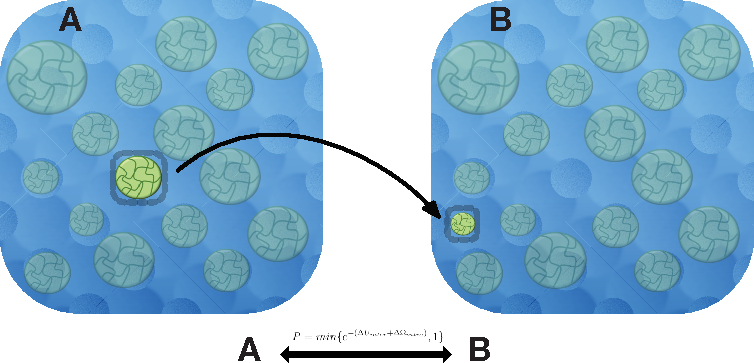
\includegraphics[width=0.75\textwidth]{Figures/modelos/mc_model.pdf}
		\caption{Esquema de un paso en el algoritmo de Metropolis-Monte Carlo. El paso de un estado \textbf{A} a uno \textbf{B} esta mediado por el cambio de energ\'ia entre ambas configuraciones. }
		\label{fig:mc:pasos_mc}
	\end{figure}
	
	La probabilidad de aceptar o no dichos cambios en el sistema viene dado por:
	
	\begin{align}
		P_{A \to B} = min \{e^{-(\beta\Delta U_{inter} +\beta \Delta \Omega_{intra})},1\}
		\label{eq:mc:probabilidad}
	\end{align}
	
%	\noindent en donde $\Delta U_{inter}$ y $\Delta\Omega_{intra}$ son los cambios en energ\'ia libre de los estados inicial y final. 
	
		De la  ecuaci\'on \ref{eq:mc:probabilidad} puede notarse que, si el cambio de energ\'ia libre es negativo, es decir, se pasa a un estado m\'as estable, este paso es aceptado autom\'aticamente. Se obtiene una probabilidad de uno. 
	
	
	Si por el contrario el cambio de energ\'ia libre es desfavorable, es decir, $\beta\Delta U_{inter} + \beta\Delta \Omega_{intra} > 0$, la probabilidad de aceptar el paso es menor a uno. En este caso, se sortea un n\'umero aleatorio y, si este es menor o igual a la probabilidad de aceptaci\'on, el paso se acepta. De lo contrario, se rechaza. 
	

	
	\section{Nanogel de P(NIPAm-MAA) en soluci\'on diluida: fluctuaciones de volumen} \label{sec:fluctuacion-volumen}
	
	El estudio de las soluciones de nanogeles necesita una caracterizaci\'on previa y comprensi\'on de los sistemas aislados, en particular nos interesa caracterizar la fluctuaci\'on en volumen que pueden tener estos sistemas al varias las condiciones de su entorno.  Es posible sustraer esta informaci\'on a partir del potencial termodin\'amico de un nanogel aislado en soluci\'on.
	
	%El c\'alculo de su potencial termodin\'amico y c\'omo puede usarse para estudiar las fluctuaciones en volumen de estos sistemas aislados.
	La respuesta a est\'imulo se estudi\'o en detalle en la referencia \cite{perez2021thermodynamic}, donde adem\'as de observar los cambios en el pH, temperatura y concentraci\'on de sal, se estudia c\'omo son modificadas sus propiedades con la estructura del microgel, es decir la arquitectura de la red polim\'erica: distribuci\'on de los mon\'omeros que poseen respuesta a est\'imulo.
	
	El nanogel considerado en este estudio posee $N_{seg} = 5 \times 10^4$ segmentos con $n_{ch} = 500$ segmentos por cadena, las cuales tienen un 35\% de MAA en su estructura polim\'erica, $x_{MAA} = 0.35$. El 65\% restante est\'a compuesto por mon\'omeros de NIPAm.
	
	En la figura \ref{fig:mc:energy-intra}, se observa el potencial termodin\'amico asociado a un nanogel aislado en funci\'on de su radio. Las curvas presentadas corresponden a tres concentraciones salinas. El pH del sistema es 4.65, el cual coincide con el pKa intr\'inseco del mon\'omero de MAA aislado. La temperatura para este sistema es de $25 ^\circ C$. De cada una de las curvas se obtiene el m\'inimo local/total de la energ\'ia intramolecular de un nanogel aislado. Este m\'inimo energ\'etico corresponde al radio \'optimo del nanogel aislado. Se puede notar que hay un aumento en el radio \'optimo del nanogel a medida que disminuye la concentraci\'on salina.
	
	Bajo condiciones de pH 4.65, hay una fracci\'on de segmentos de MAA cargados el\'ectricamente dentro de la red polim\'erica; en consecuencia, esta se expande para disminuir las repulsiones electrost\'aticas. Dicho efecto se magnifica con la disminuci\'on de la concentraci\'on de sal, la cual proporciona contraiones que apantallan las cargas del pol\'imero. Este resultado fue reportado en \cite{perez2021thermodynamic} y discutido en el cap\'itulo \ref{Chapter-geles} sobre el rol que cumple la concentraci\'on salina como est\'imulo de los hidrogeles polim\'ericos.
	
	
	\begin{figure}[!htb]
		\centering
		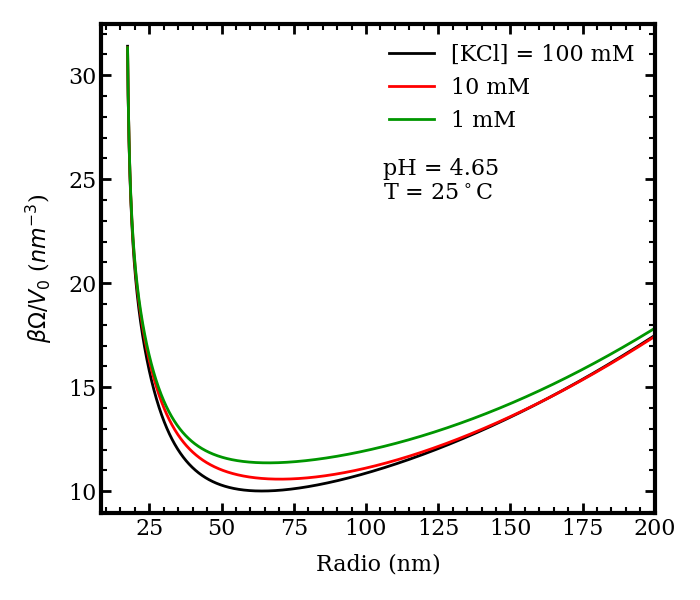
\includegraphics[width=0.45\textwidth]{Figures/graph-mc/interna.png}
		\caption{Energ\'ia libre de un nanogel aislado en funci\'on del tama\~no del mismo. Las curvas corresponden a diferentes condiciones salinas. El pH de la soluci\'on es de 4.65 y la temperatura $25 ^\circ C$. $\Omega_{MG}$, esta en unidades convenientes, donde $V_0=\frac{4}{3}\pi R_0^3$ es el volumen de la part\'icula polim\'erica seca y $\beta = \frac{1}{k_B T}$}
		\label{fig:mc:energy-intra}
	\end{figure}
	
	
	La figura \ref{fig:mc:energy-intra} nos muestra la energ\'ai libre interna de un nanogel aislado  para diferentes concentraciones salinas, el pH corresponde al pKa aparente del MAA, 4.65. 
	La energ\'ia libre es obtenida a trav\'es de un potencial termodin\'amico descrito en la secci\'on \ref{sub:mc:omega}, el mismo ser\'a usado para el calculo de las fluctuaciones en volumen que presente sistema: nanogel aislado.
	\subsection{Fluctuaciones en volumen}\label{sec:mc:fluctuacion}
	
La fluctuaci\'on de volumen es una variaci\'on del volumen de un sistema, son una medida de la estabilidad del tama\~no de un nanogel. A menor  fluctuaci\'on, mayor es la estabilidad.
	Se puede calcular la fluctuaci\'on en volumen mediante \cite{callen1991thermodynamics}:
	
	\begin{align}
		\frac{\Delta V}{V} = \sqrt{\frac{k_BT}{V}\kappa_T}
	\end{align}
	
	\noindent en donde $\Delta V$ es la varianza del volumen del nanogel que se define como:
	\begin{align}
		\Delta V = \sqrt{\langle V^2\rangle - \langle V \rangle^2}
	\end{align}
	Adem\'as, $V$ es el volumen medio y $\left< V^2\right>$  es el volumen cuadr\'atico medio del nanogel y $\kappa_T$ es la incompresibilidad isot\'ermica del sistema. Es una medida de la resistencia a la compresi\'on del sistema. A mayor $\kappa_T$, mayor rigidez.
	Se define como la relaci\'on entre la variaci\'on de presi\'on y  volumen de un fluido a temperatura constante, considerando nuestro potencial termodin\'amico, $\Omega_{NG}$, se puede obtener la siguiente forma:
	
	
	\begin{align}
		\begin{aligned}
			\kappa_T & = -\frac{1}{V} \left( \frac{\partial V}{\partial P}\right)_T \\
			& =\frac{1}{V} \left( \frac{\partial^2 \Omega_{NG}}{\partial V^2}\right)^{-1}_T \\
			& \kappa_T  = 12 \pi R_{eq} \left( \frac{\partial^2 \Omega_{NG}}{\partial R^2}\right)^{-1}_{T,R=R_{eq}}
		\end{aligned}
	\end{align}
	\noindent en la cual $R_{eq}$ hace referencia al radio de equilibrio, es decir al m\'inimo de las curvas de la energ\'ia $ \Omega_{NG}$, presentadas en \ref{fig:mc:energy-intra}. Todas las dem\'as variables fueron previamente definidas en la secci\'on \ref{sec:mc:energia_intra}
	
	\begin{figure}
		\centering
		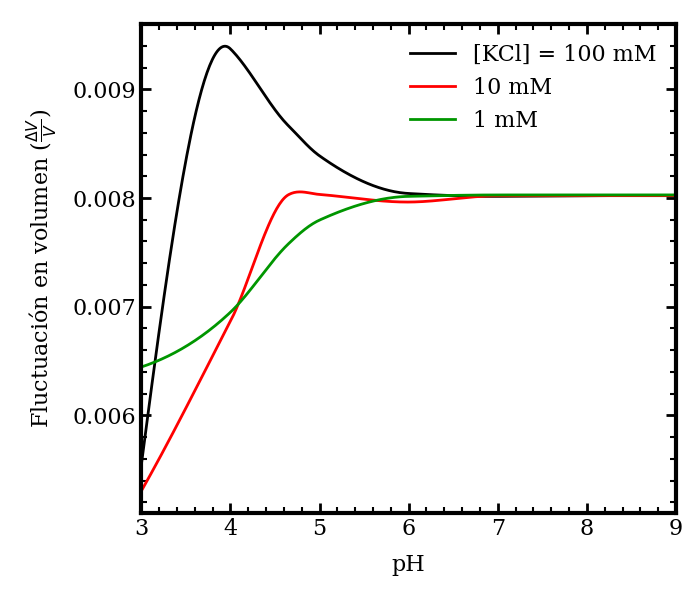
\includegraphics[width=0.45\linewidth]{Figures/graph-mc/fluct-pH.png}
		\caption{Gr\'afico de la fluctuaci\'on en volumen de un nanogel aislado. El nanogel esta compuesto por $5\times 10^4$ segmentos (mon\'omeros) repartidos en cadenas de 500 segmentos cada una}
		\label{fig:mc:flut-pH}
	\end{figure}
	
	En la figura \ref{fig:mc:flut-pH} se observa la fluctuaci\'on de un nanogel aislado en funci\'on del pH de la soluci\'on. Se presentan curvas correspondientes a tres condiciones salinas: 1, 10 y 100 mM en KCl. La temperatura es de 25$^\circ$C, condiciones en las cuales el PNIPAm posee un comportamiento hidrof\'ilico. Es decir, en estas condiciones, las fluctuaciones de tama\~no no se ven afectadas por el rol cr\'itico de la hidroficidad.
	En t\'erminos generales, se observa que la fluctuaci\'on relativa del sistema a las diferentes condiciones presentadas es del orden de $10^{-3}$. Sin embargo, dentro de estos valores, se puede notar un aumento de la fluctuaci\'on al aumentar el pH hasta estabilizarse en valores de pH mayores a 6.
	A bajos valores de pH, el nanogel no posee carga el\'ectrica, ya que los mon\'omeros de MAA que componen la red polim\'erica se encuentran protonados (estamos por debajo del pKa intr\'inseco del MAA). En estas condiciones, un cambio en el tama\~no del nanogel requiere cambios en la energ\'ia libre  dada por la adsorci\'on de solvente y de los iones presentes en el sistema, adem\'as de la contribuci\'on el\'astica que conlleva el cambio de radio.
	Con el aumento en el grado de carga de la red polim\'erica se esperar\'ia una entrada de contraiones. A valores por debajo del $pK_a$ intr\'inseco del MAA la red polim\'erica que compone al nanogel no posee carga el\'ectrica, en consecuencia las fluctuaciones son bajas. A pH alto se obtiene el mayor grado de carga posible, sin cambios en la carga el\'ectrica del pol\'imero, las fluctuaciones de volumen se estabilizan.
	
	En particular, una alta concentraci\'on salina promueve la desprotonaci\'on de los segmentos de MAA para peque\~nos aumentos de pH. Esto se debe a que los iones presentes en la soluci\'on pueden apantallar la carga el\'ectrica adquirida por los grupos carbox\'ilicos de los mon\'omeros de MAA. Como resultado, la entrada de iones favorece la fluctuaci\'on en volumen del nanogel.
	A medida que aumenta el pH, m\'as unidades de MAA adquieren carga el\'ectrica, por lo cual un cambio en su volumen se ve favorecido. Para minimizar las repulsiones el\'ectricas de la red polim\'erica, el nanogel puede expandirse o adsorber m\'as cantidad de contraiones presentes en la soluci\'on. Como resultado, se observa un aumento en la fluctuaci\'on del volume de la part\'icula, el cual se intensifica con el aumento de la concentraci\'on salina.
	
	%%%%%%%%%%%%%%%%%%
	A pH 7, el nanogel se encuentra completamente desprotonado, cargado el\'ectricamente. La fluctuaci\'on del sistema es mayor y se estabiliza como consecuencia de que no es posible un cambio en el grado de carga el\'ectrica del nanogel. 
	En una situaci\'on de pH intermedios, la desprotonaci\'on es incompleta y el nanogel puede expandirse o contraerse, por lo cual la fluctuaci\'on en el sistema es la mayor de todas.
	
	%%%%%%%%%%%%%%%%%%%%%%%%%%%
	
	En la figura \ref{fig:mc:fluct-T} se muestra el efecto de la temperatura en las fluctuaciones en el volumen del nanogel. Se presentan tres curvas correspondientes a tres valores caracter\'isticos de pH: por debajo y por encima del $pK_a$ intr\'inseco del MAA, pH 3 y 7, respectivamente, y pH 4.65, igual al pKa del MAA aislado.
	
	A pH 3 el nanogel no posee carga el\'ectrica, y como mencionamos antes, las fluctuaciones son bajas. El aumento de \'estas es por efecto del cambio de la temperatura, en particular por el cambio en la hidroficidad de PNIPAm. Sin embargo, no se observan cambios apreciables a medida que se aumenta la temperatura del sistema, incluso cerca de la temperatura de transici\'on del PNIPAm, alrededor de los 32$^\circ$C. Por arriba de esta temperatura, el nanogel adopta un estado colapsado y no hay ninguna fuerza impulsora que promueva un cambio en su volumen.
	%%%%%%%%%%%%%%
	%%% 
	
	En la misma figura, \ref{fig:mc:fluct-T}, a valores de pH 4.65 y 7, los mon\'omeros de MAA se encuentran  desprotonados, la red polim\'erica adquiere carga el\'ectrica. 
	A temperatura baja las fluctuaciones son mayores que a pH 3 por efecto de la desprotonaci\'on de la red polim\'erica. En particular las fluctuaciones son mayores a pH 4.65 dado que es posible una regulaci\'on de carga el\'ectrica, a pH 7 todos los segmentos de MAA se encuentran mayormente desprotonados.
	Con el aumento de temperatura hay un aumento de las fluctuaciones del sistema.
	Esto ocurre hasta llegar a la temperatura caracter\'istica de transici\'on volum\'etrica del PNIPAm, al seguir aumentando la temperatura se origina un colapso en la estructura del nanogel, siendo las interacciones entre los segmentos de NIPAm las predominantes y estabilizando un tama\~no espec\'ifico del nanogel.
	Las fluctuaciones en este cambio de fase volum\'etrico son las mayores. Pasada la transici\'on las fluctuaciones decaen a los valores m\'as bajos posibles.
	
	
	%%%%%%%%%%%%%%%%%%%%%%%%%%	
	
	\begin{figure}
		\centering
		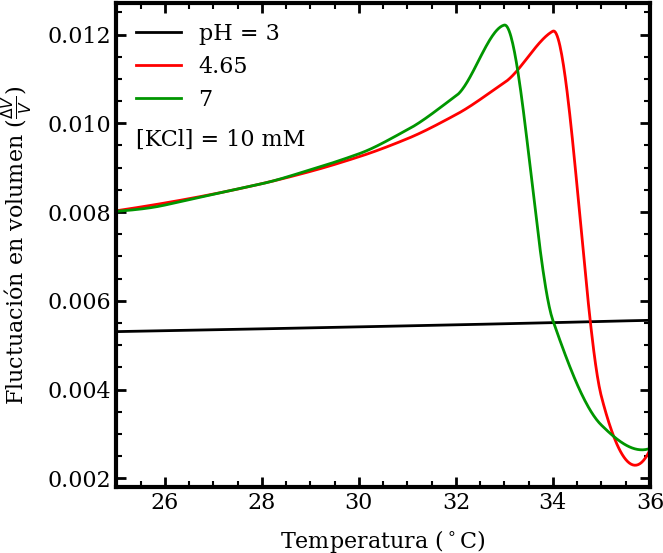
\includegraphics[width=0.45\linewidth]{Figures/graph-mc/fluct-T.png}
		\caption{Gr\'afico de la fluctuaci\'on en volumen de un nanogel aislado. El nanogel esta compuesto por $5\times 10^5$ segmentos (mon\'omeros) repartidos en cadenas de 500 segmentos cada una.}
		\label{fig:mc:fluct-T}
	\end{figure}
	
	
	%%%%%%%%
	El estudio de las fluctuaciones en volumen de estos sistemas aislados nos muestran la baja magnitud de las mismas. No hay una fuerza impulsora significativa para que los nanogeles cambien su volumen. Esto puede traducirse en que en una soluci\'on coloidal, diluida, la poblaci\'on de tama\~nos de nanogeles sea \'unica o con muy poca dispersi\'on. 
	
	En la siguiente secci\'on se mostrar\'an los resultados de soluciones de nanogeles, desde concentraciones diluidas hasta concentradas.
	Se ver\'a cu\'al es el rol de las interacciones entre las part\'iculas y si se mantiene o no la tendencia de las fluctuaciones en volumen encontrada en esta secci\'on.
	
	\section{Resultados: Soluciones de nanogeles polim\'ericos}
	
	En esta secci\'on mostraremos los resultados obtenidos en el estudio sistem\'atico de tres soluciones de nanogeles compuestos por segmentos de N-isopropilamina y \'acido metacr\'ilico. La red polim\'erica, P(NIPAm-MAA), posee un 35\% de MAA. Para cada una de estas soluciones, se estudiaron su respuesta a cambios en el pH, la temperatura y la concentraci\'on salina. En cada caso, se comparar\'a con un nanogel a diluci\'on infinita, como lo discutimos en el cap\'itulo \ref{Chapter-geles} de esta tesis. Las soluciones consideras corresponden a 0.10 mg/ml, 1.0 mg/ml y 5.0 mg/ml  de nanogeles las cuales fueron seleccionadas para representar una soluci\'on de nanogeles diluida, una relativamente concentrada y una muy concentrada.
	
	Como mencionamos en la secci\'on \ref{sec:mc:mc}, la metodolog\'ia utiliza simulaciones Monte Carlo. Estas se componen de $5\times 10^6$ pasos; cada paso de simulaci\'on se compone de una compresi\'on/expansi\'on y cambio de posici\'on espacial de una part\'icula que compone la soluci\'on. La caja de simulaci\'on contiene 100 part\'iculas. Los par\'ametros de construcci\'on de cada nanogel han sido especificados en la secci\'on \ref{sec:fluctuacion-volumen}: Nanogeles con $N_{seg} = 5 \times10^4$ segmentos y $n_{ch} = 500$ segmentos por cadena. Un estudio sistem\'atico de las fluctuaciones en volumen de estos nanogeles mostraron que sus fluctuaciones de volumen son muy peque\~nas ($\approx$ 0.1 $\%$). %En este sentido, para observar efectos en la concentraci\'on de estas part\'iculas, es necesario poseer fluctuaciones lo m\'as grandes posibles.
	
	
	
	\subsection{Efecto de la concentraci\'on de nanogeles}
	En la figura \ref{fig:mc:densidad-probabilidad} se muestra la densidad de probabilidad de tama\~nos (radios) de tres soluciones de nanogeles. Las condiciones del bulk de cada una de las soluciones corresponden a una temperatura de 25$^\circ$C y una concentraci\'on de $[KCl]$ de 1 mM, en cada panel se muestra un pH de estudio distinto, 3, 4.65, y 5 y 7 para los paneles A, B, C y D respectivamente. Estos valores son considerados por estar por debajo (pH 3) y por arriba (pH 5) del pKa intr\'inseco de los mon\'omeros de MAA (pH 4.65) y condiciones de neutralidad (pH 7), que son condiciones cercanas al pH fisiol\'ogico. Las diferentes curvas dentro de cada panel representan una concentraci\'on de nanogeles diferente, 0.10, 1.0 y 5.0 mg/ml.
	
	\begin{figure}
		\centering
		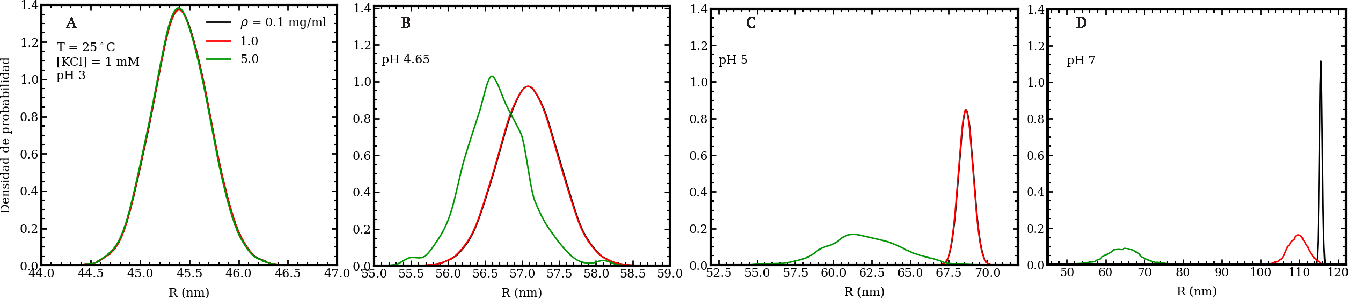
\includegraphics[width=0.99\linewidth]{Figures/graph-mc/sizes-phs.pdf}
		\caption{Densidad de probabilidad de tama\~no para tres diferentes soluciones de nanogeles 0.1, 1.0 y 5.0 mg/ml. Cada panel corresponde a un pH de trabajo diferente: 3, 4.65, 5.50 y 7 para los paneles A, B, C, y D respectivamente. Otras condiciones de trabajo son: temperatura 25$^\circ$C y 1 mM  [KCl].}
		\label{fig:mc:densidad-probabilidad}
	\end{figure}
	
	La figura \ref{fig:mc:densidad-probabilidad} nos muestra, de forma general, que los perfiles de densidad de probabilidad en tama\~no de los nanogeles var\'ia con su concentraci\'on y el pH del medio. Se puede observar que el aumento del pH desplaza las curvas hacia valores mayores de radio. Esto se puede explicar por el aumento en el n\'umero de segmentos de MAA que se desprotonan a medida que se aumenta el pH. En la secci\'on \ref{sec:mc:phs_salt_temp} daremos una explicaci\'on m\'as detallada de este fen\'omeno.
	
	Observando la figura \ref{fig:mc:densidad-probabilidad}A notamos que todas las concentraciones de nanogeles exhiben picos definidos, lo que sugiere una distribuci\'on de tama\~no m\'as uniforme. La dispersi\'on de radios es de 2 nm aproximadamente (el ancho de la distribuci\'on). Bajo estas condiciones no se aprecia ninguna fuerza impulsora que modifique significativamente el tama\~no de los nanogeles, de hecho no se puede apreciar una diferencia importante entre cada una de las soluciones de las part\'iculas.
	
	A medida que el pH aumenta a 4.65, figura \ref{fig:mc:densidad-probabilidad}B, la distribuci\'on correspondiente a una concentraci\'on de 5 mg/ml se diferencia de las otras dos. El desplazamiento es hacia menores valores de radio. Esta separaci\'on es aun mayor a medida que se aumenta el pH, panel C. Finalmente en la figura \ref{fig:mc:densidad-probabilidad}D a pH 7, las diferencias entre las concentraciones se incrementan hasta observar una separaci\'on entre todas las concentraciones de nanogeles consideradas. Esta disminuci\'on del tama\~no se explica al considerar los potenciales de interacci\'on entre part\'iculas. Para disminuir la energ\'ia dada por estas interacciones, los nanogeles buscan disminuir su tama\~no, si bien esto conlleva un aumento en la energ\'ia libre interna del nanogel, ver figura \ref{fig:mc:energy-intra}, el aumento de la energ\'ia libre interna es menor que el producido por las interacci\'on intermoleculares. A medida que disminuimos la concentraci\'on de nanogeles el espacio disponible en soluci\'on aumenta, teniendo mayor libertad para  aumentar su tama\~no y de esta forma acercarse m\'as a su radio ideal. A  diluci\'on infinita las  interacciones entre part\'iculas son exactamente cero y el radio optimiza el potencial termodin\'amico interno. 
	
	La capacidad de fluctuaci\'on de tama\~no de los nanogeles es fuertemente afectada por la capacidad de los nanogeles de interactuar con vecinos, lo cual est\'a interrelacionado con la concentraci\'on de la soluci\'on.
	En ese sentido, la figura \ref{fig:mc:rdf} muestra la distribuci\'on radial para las tres diferentes soluciones de nanogeles. Consideramos las mismas condiciones del bulk de la figura \ref{fig:mc:densidad-probabilidad}B, es decir, pH 4.65, temperatura de 25$^\circ$C y concentraci\'on salina de 1 mM.
	
	Observamos que la soluci\'on con concentraci\'on m\'as alta de nanogeles ($\rho$ = 5.0 mg/ml) exhibe un perfil de distribuci\'on radial caracter\'istico de sistemas l\'iquidos, donde se pueden distinguir picos marcados en la distribuci\'on que indican una estructura ordenada a corta distancia, lo que sugiere una disposici\'on uniforme de las primeras part\'iculas vecinas dentro de la soluci\'on.
	
	Por otro lado, las soluciones m\'as diluidas ($\rho$ = 0.10 y 1.0 mg/ml) muestran un perfil que alcanza  un m\'aximo y manteni\'endose as\'i con peque\~nas variaciones. Este comportamiento es t\'ipico al de un sistema gaseoso (diluido), donde la distribuci\'on de part\'iculas es  aleatoria y menos estructurada.
	
	%Estos resultados  indican que las interacciones entre los nanogeles son m\'as frecuentes en soluciones de mayor concentraci\'on. En contraste, bajas concentraciones de part\'iculas, indican menos interacciones, los nanogles est\'an m\'as espaciados, reflejando un sistema con menor cantidad de interacciones entre part\'iculas.
	
	\begin{figure}
		\centering
		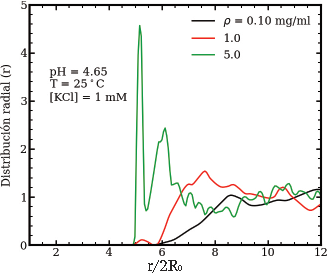
\includegraphics[width=0.45\linewidth]{Figures/graph-mc/rdf.pdf}
		\caption{Funci\'on de distribuci\'on radial para las tres soluciones de nanogeles. Las curvas corresponden a las tres concentraciones de naogeles consideradas: 0.10, 1.0, 5 mg/ml. Las condiciones del bulk de la soluci\'on son pH 4.65, [KCl] = 1 mM, la temperatura del sistema es 25$^\circ$C. En el eje x se ha usado el valor de radio seco, $R_0 = 10 $ nm, de los nanogeles para usar unidades reducidas en la distancia nanogel-nanogel.}
		\label{fig:mc:rdf}
	\end{figure}
	
	
	
	\subsection{Respuesta a est\'imulos: pH, concentraci\'on salina y temperatura.}\label{sec:mc:phs_salt_temp}
	
	\textbf{Respuesta a cambios en pH}
	
	En esta secci\'on estudiamos la influencia de la concentraci\'on de los nanogeles en su respuesta a est\'imulos, en particular los resultados que mostramos m\'as abajo surgen de los cambios en el pH, la concentraci\'on salina y la temperatura. En primera instancia, veremos c\'omo se comportan las soluciones con la variaci\'on del pH. %Teniendo en cuenta que las soluciones de nuestros nanogeles est\'an influenciadas por su concentraci\'on, veremos c\'omo estas soluciones 
	
	La Figura \ref{fig:mc:xvspH} ilustra la respuesta de las soluciones cuando son sometidas a cambios en el pH. Se destacan el tama\~no promedio $\left<R\right>$, el grado de disociaci\'on $\left<f\right>$ y la fracci\'on en volumen $\left<\phi\right>$, correspondientes a los paneles A, B y C, respectivamente. A una temperatura de 25$^\circ$C y con una concentraci\'on de $[KCl]$ de 1 mM, se observa principalmenteel efecto de la desprotonaci\'on de los segmentos de MAA, dado que las unidades de NIPAm son hidrof\'ilicas bajo estas condiciones.
	El calculo  del radio medio de los nanogeles se realiz\'o a trav\'es de :
	\begin{align}
		\left< R\right> = \int R\delta(R)dR
	\end{align} 
	
	\noindent en donde, $R$ es el radio de la part\'icula de nanogel. La densidad de probabilidad de tama\~no es $\delta(R)$, la cual es obtenida de la figura \ref{fig:mc:densidad-probabilidad}. 
	La cantidada $\left<\phi\right>$ se define como la fracci\'on en volumen  de la soluci\'on ocupada por los nanogeles.
	
	 Se han analizado tres concentraciones distintas de nanogeles, $\rho$ = 0.10, 1.0 y 5.0 mg/ml, para estudiar el efecto de la concentraci\'on. En los paneles A y B, las curvas punteadas representan el comportamiento en un sistema de diluci\'on infinita.
	
	\begin{figure}[!htb]
		\centering
		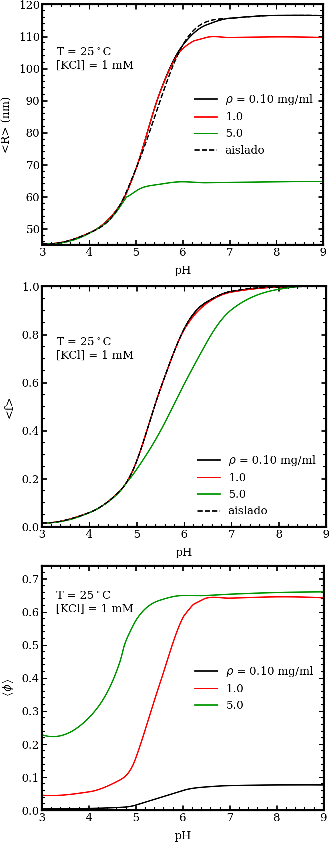
\includegraphics[width=0.4\linewidth]{Figures/graph-mc/xvspH.pdf}
		\caption{Variaci\'on de las propiedades medias de la soluci\'on de nanogeles en funci\'on del pH de trabajo. El panel A muestra el tama\~no $\left<R\right>$, el B el grado de carga $\left<f\right>$ y el C la fracci\'on en volumen $\left<\phi\right>$. La temperatura es de 25$^\circ$C y la concentraci\'on salina de 1 mM en $[KCl]$. Cada curva corresponde a un grado de empaquetamiento. Los nanogeles aislados se muestran en los paneles A, B y C.}
		\label{fig:mc:xvspH}
	\end{figure}
	
	El radio medio de los nanogeles crece con el aumento del pH, independientemente de la concentraci\'on contemplada en nuestro estudio. Esto se explica por la  influencia del pH en la carga el\'ectrica de los segmentos de MAA: a un pH m\'as elevado, m\'as segmentos de MAA se desprotonan, incrementando la carga el\'ectrica negativa del nanogel. En el panel B (\ref{fig:mc:xvspH}B), se observa que el aumento del pH tambi\'en eleva el grado de disociaci\'on de los segmentos de MAA. Este crecimiento en tama\~no es resultado de las repulsiones electrost\'aticas en la red polim\'erica de los nanogeles, como reportaron \citet{perez2021thermodynamic}, donde se indica que estas repulsiones disminuyen al distanciar los centros de carga de la estructura del nanogel.
	
	El efecto de la concentraci\'on de los nanogeles se evidencia al examinar las distintas curvas en cada pane. El comportamiento de la soluci\'on m\'as diluida, 0.10 mg/ml, es similar al del sistema aislado en todo el rango de pH. La concentraci\'on intermedia, 1.0 mg/ml, presenta un comportamiento parecido, aunque muestra diferencias alrededor de pH 6. En contraste, la soluci\'on m\'as concentrada, 5.0 mg/ml, solo se asemeja al sistema aislado a pH inferiores a 5, en ausencia de carga el\'ectrica.
	
	En t\'erminos generales, al aumentar la concentraci\'on de nanogeles, se observa una reducci\'on en la respuesta esperada de un sistema aislado, con una disminuci\'on de m\'as del 40\% para la soluci\'on m\'as concentrada. A diferencia de un sistema aislado, las soluciones de nanogeles presentan interacciones energ\'eticas intermoleculares, dadas por los potenciales de Hertz y Yukawa. Estas diferencias en tama\~no o grado de carga se explican por las interacciones entre ellos. Esto se hace evidente al observar la figura \ref{fig:mc:xvspH}C, en la cual se muestra c\'omo cambia la fracci\'on en volumen con respecto al cambio de pH, aumentando r\'apidamente con este y a\'un m\'as para concentraciones m\'as altas. Una fracci\'on en volumen m\'as alta implica una mayor interacci\'on entre las part\'iculas, con las part\'iculas ocupando una mayor fracci\'on en volumen de la soluci\'on, la proximidad entre ellas disminuye, lo que intensifica su interacci\'on.
	
	Los potenciales de Hertz y Yukawa, detallados en la secci\'on \ref{sec:mc:energia_intra}, nos modelan  la capacidad de deformarse, por solapamiento, y las interacciones de largo alcance, respectivamente y son los responsables de la energ\'ia de interacci\'on entre los nanogeles de la soluci\'on. Aumentando la energ\'ia con la concentraci\'on de las soluciones.
	Para reducir esta energ\'ia de interacci\'on, a concentraciones altas,  las part\'iculas adquieren un tama\~no menor al esperado en un sistema aislado. Esta diferencia con respecto al sistema aislado conlleva un incremento en la energ\'ia libre interna de los nanogeles, pero se compensa con una disminuci\'on en la energ\'ia de interacci\'on. Este efecto se amplifica con el aumento en la concentraci\'on, como se observa en las diferentes curvas de la figura \ref{fig:mc:xvspH}A. 
	Adicionalmente la disminuci\'on en el tama\~no de los nanogeles afecta su grado de carga, generando un efecto entr\'opico que impulsa a los iones a salir de los entornos confinados de los nanogeles de menor tama\~no hacia la soluci\'on, lo que a su vez reduce el apantallamiento en los segmentos de MAA desprotonados. La energ\'ia libre qu\'imica necesaria para desprotonar los segmentos de MAA es mayor, lo que se traduce en un desplazamiento hacia valores m\'as altos de pH para alcanzar el mismo grado de carga que un sistema ideal.
	
	\textbf{Respuesta a cambios en la concentraci\'on salina}
	
	La figura \ref{fig:mc:reentrante} exhibe el comportamiento del tama\~no medio $\left<R\right>$ de los nanogeles en funci\'on de la concentraci\'on salina a un pH de 4.65 y 7, paneles A y B respectivamente, la temperatura del sistema es de 25$^\circ$C. Las curvas s\'olidas representan las tres concentraciones de nanogeles $\rho =$ 0.1, 1.0 y 5.0 mg/ml, mientras que la l\'inea punteada muestra la respuesta de un nanogel aislado. En ambos paneles se observa una transici\'on reentrante caracter\'istica, donde inicialmente el tama\~no de los nanogeles aumenta con la concentraci\'on salina hasta un m\'aximo, antes de disminuir el tama\~no de las part\'iculas. Este fen\'omeno se atribuye a la interacci\'on entre los mon\'omeros cargados y la adsorci\'on de contraiones provenientes del KCl. Bajo estas condiciones de pH (ya sea 4.65 o 7) hay una proporci\'on de los segmentos de MAA que se encuentran desprotonados, vease la figura \ref{fig:mc:xvspH}B, con mayor magnitud a pH 7. A bajas concentraciones salinas, el apantallamiento sobre estos segmentos cargados el\'ectricamente es insuficiente, lo que conlleva a un aumento del tama\~no de los nanogeles para minimizar las repulsiones electrost\'aticas. Si se aumenta la concentraci\'on de contraiones, en primera instancia se favorece la protonaci\'on de los segmentos de MAA \cite{perez2021thermodynamic}, provocando un aumento del \textit{swelling} de los nanogeles presentes en la soluci\'on. Con una mayor concentraci\'on de sal, el incremento en la adsorci\'on de contraiones  conduce a un mejor apantallamiento de los contraiones, reduciendo las repulsiones entre los segmentos de MAA desprotonados. En este punto se esperar\'ia que este aumento en el apantallamiento de las cargas permita que m\'as segmentos se desprotonen y se aumente a\'un m\'as el radio de las part\'iculas, sin embargo, el efecto observado es el contrario: compresi\'on de la estructura de los nanogeles. El exceso de contraiones en el interior de los nanogeles tiene como consecuencia que las interacciones electrost\'aticas se vuelvan de menor alcance efectivo, permitiendo que los centros de carga puedan acercarse mucho m\'as, lo que facilita una relajaci\'on y disminuci\'on en la energ\'ia el\'astica de los nanogeles. Esta transici\'on reentrante es m\'as evidente a pH 7 donde los segmentos de MAA desprotonados (con carga el\'ectrica) son mayor\'ia.
	
	\begin{figure}
		\centering
		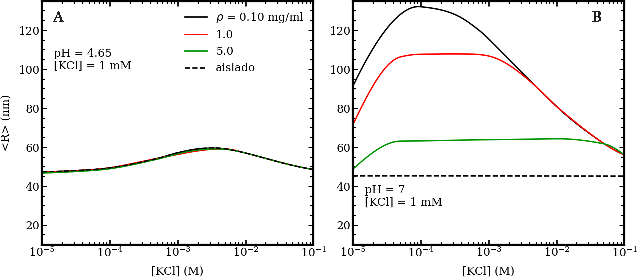
\includegraphics[width=0.99\linewidth]{Figures/graph-mc/r-salts-pHs.pdf}
		\caption{Variaci\'on del radio medio ($\left<R\right>$) con la concentraci\'on de sal para diferentes concentraciones de nanogeles. El pH es 4.65 y 7 para el panel A y B respectivamente. La temperatura del sistema es de 25$^\circ$C. Las curvas s\'olidas corresponden a $\rho=$ 0.10, 1.0 y 5.0 mg/ml de nanogeles, y a trazos se incorpora la respuesta de un nanogel aislado.}
		\label{fig:mc:reentrante}
	\end{figure}
	
En la figura \ref{fig:mc:reentrante} se puede observar que a medida que aumenta la concentraci\'on de nanogeles, menor es la respuesta de estas part\'iculas a cambios en la concentraci\'on salina. Esto \'ultimo se evidencia mejor en la figura \ref{fig:mc:reentrante}B a un pH de 7. En estas condiciones, el tama\~no y grado de carga de estas part\'iculas est\'an bien diferenciados, figura \ref{fig:mc:xvspH}A y B. La diferencia se puede atribuir al costo energ\'etico de las interacciones entre nanogeles, el cual es compensado con un menor tama\~no de los mismos. Una mayor vecindad de nanogeles, (ver figura \ref{fig:mc:rdf}), hace que interact\'uen a\'un m\'as entre ellos, aumentando la energ\'ia intermolecular del sistema. Al igual que en la figura \ref{fig:mc:xvspH}, es la energ\'ia libre interna de los nanogeles la que aumenta como consecuencia de poder reducir la energ\'ia atribuida a las interacciones que nos explican losgit p potenciales de Hertz y Yukawa. A medida que se diluye lo suficiente la soluci\'on, nos acercamos al comportamiento ideal, es decir, un nanogel aislado donde las part\'iculas pueden aumentar su tama\~no para reducir su energ\'ia libre interna sin mayor costo en las interacciones intermoleculares.
	
	
	\textbf{Respuesta a cambios de temperatura}

A continuaci\'on presentamos el an\'alisis sobre la respuesta de nuestras soluciones de nanogeles cuando se les aplica  cambios en la temperatura. En este sentido, en la figura \ref{fig:mc:dfs_energy} se muestra la energ\'ia libre interna de un nanogel aislado en funci\'on de su tama\~no. A su vez las diferentes curvas corresponden a diferentes temperaturas. En el panel A se trabaja con un pH  de 4.65,  en esta primera figura podemos observar c\'omo al aumentar la temperatura se origina un nuevo m\'inimo en la energ\'ia libre a valores m\'as peque\~nos de radio. Un desplazamiento de radios alrededor de los 60 nm hacia valores de 12 nm. Este cambio se explica por el efecto de hidrofobicidad del PNIPAm que compone la red de los nanogeles. El m\'inimo global se va profundizando al aumentar la temperatura, por lo que es de esperar un estado colapsado bien definido al aumentar la temperatura de las soluciones de part\'iculas consideradas en este estudio. 
Por otro lado, en el panel B se considera un pH de 7, a diferencia del panel A, vemos que la aparici\'on de un m\'inimo a bajos radios coexiste con un estado expandido del nanogel. A temperaturas bajas, el m\'inimo energ\'etico correspondiente al estado colapsado es un m\'inimo local, y su estado expandido correponde al m\'inimo global de la energ\'ia libre. Al aumentar la temperatura se observa un intercambio gradual entre estos dos estados. Esta coexistencia de m\'inimos de la energ\'ia libre se debe a que a pH 7 existe una buena proporci\'on de segmentos de MAA desprotonados, con lo cual las repulsiones electrost\'aticas entre estos segmentos favorecen, a bajas temperaturas, un estado expandido, mientras que a temperaturas altas las interacciones del PNIPAm conducen a una estructura colapsada.% En la siguiente figura se presentar\'an los resultados al considerar prioritarios los dos m\'inimos de la energ\'ia libre de los nanogeles.

	
	
	\begin{figure}[!htb]
		\centering
		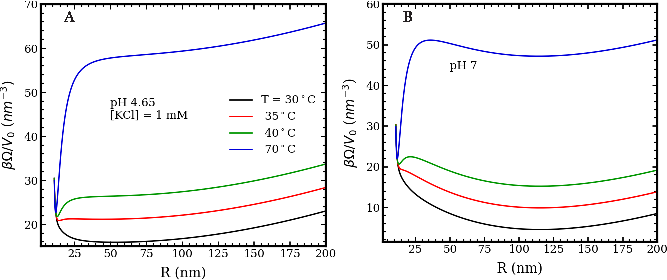
\includegraphics[width=0.99\linewidth]{Figures/graph-mc/dfs_energy.pdf}
		\caption{Energ\'ia libre interna de un nanogel aislado como funci\'on de su radio. Las diferentes curvas muestran el cambio de la energ\'ia al aumentar la temperatura, la concentraci\'on salina es 1 mM en KCl. Los paneles A y B corresponden a pH 4.65 y 7 respectivamente.}
		\label{fig:mc:dfs_energy}
	\end{figure}

	En este sentido, la figura \ref{fig:mc:temperatura-r} muestra la respuesta a los cambios de temperatura de las soluciones estudiadas considerando el comportamiento de la energ\'ia libre interna de los nanogeles, es decir la posible cohexistencia de entre nanogeles en estado expandido y colapsado. El panel A corresponde a un pH de 4.65, mientras que el panel B muestra la respuesta a la temperatura a pH 7, la concentraci\'on salina es 1 mM en KCl. Las diferentes curvas corresponden a las diferentes concentraciones de nanogeles: 0.10, 1.0 y 5.0 mg/ml, y a trazos se presenta la respuesta de un nanogel aislado.

En ambos paneles se puede apreciar c\'omo, superando cierta temperatura, los nanogeles colapsan. Esto es causado por el efecto de la temperatura sobre el PNIPAm que conforma la estructura de las part\'iculas estudiadas. Esta caracter\'istica es propia de los pol\'imeros de PNIPAm \cite{perez2021thermodynamic}, los cuales poseen una temperatura cr\'itica m\'inima de soluci\'on, que siendo superada aumenta la hidrofobicidad del PNIPAm observ\'andose un colapso en la estructura de la que forman parte. Se puede observar que una vez superada esta temperatura cr\'itica todas las concentraciones contempladas tienden al mismo estado colapsad. El radio, de aproximadamente 12 nm, que adquieren las part\'iculas es tan peque\~no que el efecto de las interacciones entre pares desaparece, predominando fuertemente solo la energ\'ia libre intramolecular de los nanogeles.

En la figura \ref{fig:mc:temperatura-r}A vemos que a condiciones de pH 4.65 no hay diferencias apreciables entre las distintas concentraciones de nanogeles y una part\'icula aislada. La diferencia en la temperatura de transici\'on de estos sistemas es insinificante. Bajo estas condiciones, pH 4.65, no hay diferencias apreciables para las tres soluciones consideradas. (v\'ease las figuras \ref{fig:mc:xvspH}A y B). El estado de carga el\'ectrica de los nanogeles en estas condiciones es el mismo. En este sentido, la fuerza impulsora, es decir, la hidrofobicidad del PNIPAm, no tiene ning\'un impedimento para llegar al deswelling del sistema y al disminuir el tama\~no de cada part\'icu, y en consecuencia reduciendo las interacciones entre nanogeles. Estos resultados son consistentes con la existencia de un solo m\'inimo en la energ\'ia libre de los nanogeles, ver figura \ref{fig:mc:dfs_energy}A. Es decir, hay una predominancia en el estado de la estructura colapsada de las part\'iculas.
	
	\begin{figure}[!htb]
		\centering
		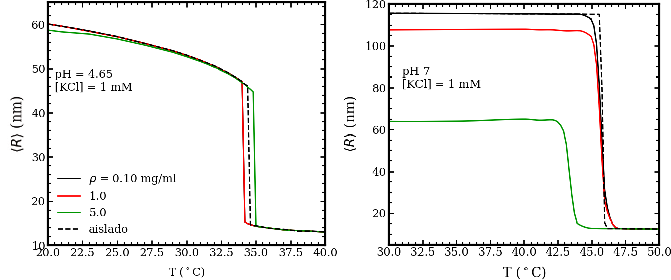
\includegraphics[width=0.99\linewidth]{Figures/graph-mc/rvst.pdf}
		\caption{Radio medio de los nanogeles en soluci\'on como funci\'on de la temperatura de la soluci\'on. pH 4.65, $[KCl]$ 1 mM. Curvas s\'olidas corresponden a concentraciones $\rho =$ 0.10, 1.0 y 5.0 mg/ml de nanogel, a trazos se presenta un sistema con una part\'icula polim\'erica aislada.}
		\label{fig:mc:temperatura-r}
	\end{figure}
	
    Continuando con nuestra descripci\'on del efecto de la temperatura, vemos en la figura \ref{fig:mc:temperatura-r}B el comportamiento de las soluciones cuando el pH de la soluci\'on tiene un valor de 7. La construcci\'on estas curvas se realiz\'o considerando la competencia entre los dos m\'inimos que surgen de la energ\'ia libre interna, ver figura \ref{fig:mc:dfs_energy}B.  Por este motivo y para poder obtener un buen barrido de los dos m\'inimos energ\'eticos se plantearon dos simulaciones para cada temperatura, cuya diferencia recae en la condiciones iniciales de las mismas. en una simulaci\'on se considera como prioritario el m\'inimo de energ\'ia libre dado por el estado colapsado y en la segunda simulaci\'on se considera el estado expandido.
Finalmente el radio medio $\left< R\right>$ para cada temperatura es obtenido:
\begin{align}
	\left< R \right> =  \left< R_s\right>\frac{e^{-\beta E_s}}{e^{-\beta E_s}+ e^{-\beta E_c}} + \left< R_c\right>\frac{e^{-\beta E_c}}{e^{-\beta E_s}+ e^{-\beta E_c}} 
\end{align}

\noindent en donde, $\left< R_s\right>$ y $\left< R_c \right>$ corresponden a los radios medios de los estados expandidos y colapsado. Adem\'as $E_s$ corresponde a la energ\'ia libre total (energ\'ia libre interna + energ\'ia intermolecular) del estado expandido, del mismo modo se define $E_c$ para el estado colapsado.

Los resutlados obtenidos, en el panel B, muestran una respuesta cualitativamente similar al panel A, el paso de un estado expandido a uno colapsado al superar una temperatura cr\'itica. No obstante podemos destacar que el estado inicial, hinchado, de las part\'iculas disminuye con el aumento de la concentraci\'on de los nanogeles. Este comportamiento se asocia a las interacciones intermoleculares descriptas por los potenciales de Hertz y Yukawa, para los cuales un aumento de la concentraci\'on significa una mayor energ\'ia de interacci\'on de a pares a medida que aumenta el tama\~no por efecto del pH (v\'ease figura \ref{fig:mc:xvspH}A) con lo cual, para minimizar la energ\'ia total del sistema, las part\'iculas adquieren un menor tama\~no respecto al esperado en un sistema aislado. Por otro lado, vemos que nuevamente el estado colapsado es igual para las tres soluciones, siendo este el mismo que para un sistema aislado.
Otro efecto causado por la concentraci\'on de part\'iculas polim\'ericas es la disminuci\'on en la temperatura de transici\'on con el aumento de la nanogeles en la soluci\'on. En particular se puede apreciar que a una concentraci\'on de 5 mg/ml se obtiene una temperatura de transici\'on menor al del sistema aislado, alrededor de 3$^\circ$C menos. El menor tama\~no medio de las part\'iculas en esta soluci\'on concentrada permite al sistema requerir menor temperatura, para alcanzar el estado colapsado. La cercania del PNIPAm  es debida al menor tama\~no por la alta densidad de nanogeles en la soluci\'on de 5 mg/ml, lo que origina interacciones m\'as efectivas entre los segmentos de NIPAm, las interacciones hidrofobicas se ven activadas por el aumento de la temperatura, alcanzando el colapso de la estructura de los nanogeles m\'as facilmente respecto al nanogel aislado.

	
	

	\section{Conclusiones}

	En este cap\'itulo se investig\'o el comportamiento de soluciones compuestas por nanogeles polim\'ericos a diferentes concentraciones. Se aplic\'o metodolog\'ia basada en simulaciones Monte Carlo. El enfoque se centr\'o en la influencia de la concentraci\'on de part\'iculas sobre la respuesta a est\'imulos de nanogeles compuestos por P(NIPAM-MAA). Se consideraron tres est\'imulos diferentes: cambios en el pH, la temperatura y la concentraci\'on de sal. Adem\'as, se estudi\'o el efecto de la concentraci\'on de nanogeles en la soluci\'on ante estos est\'imulos.
	
	Los perfiles encontrados para las distintas concentraciones de trabajo nos indican el comportamiento de un sistema relativamente diluido (concentraciones de 0.10 y 1 mg/ml), mientras que a una concentraci\'on de 5 mg/ml se observa un comportamiento m\'as cercano a un l\'iquido condesado. Para las concentraciones m\'as bajas, observamos que sus propiedades se desv\'ian m\'inimamente del sistema a diluci\'on infinita. 
	 En general, el comportamiento reportado es cualitativamente similar a un sistema con diluci\'on infinita. En particular, la respuesta a cambios de pH tambi\'en conlleva un aumento en el pKa aparente de la soluci\'on en concentraciones altas.
	
	La respuesta a la temperatura sigue los mismos lineamientos reportados en la respuesta al pH y concentraci\'on salina, es decir, un comportamiento cualitativo similar al sistema en diluci\'on infinita. En particular, a pH 4.65 no se encontr\'o diferencia alguna sobre un nanogel aislado, pero a pH 7 se reporta un comportamiento dependiente de la cantidad de nanogeles en soluci\'on. Una concentraci\'on m\'as alta permite una transici\'on de fase a menores temperaturas, as\'i como tambi\'en la obtenci\'on de menores tama\~no de part\'iculas a medida que aumenta la concentraci\'on en su estado expandido como un mecanismo para reducir la energ\'ia de interacci\'on entre los nanogeles.
	
	
	
	
	
	
	